\documentclass{article}

\usepackage{fancyhdr}
\usepackage{extramarks}
\usepackage{amsmath}
\usepackage{amsthm}
\usepackage{amsfonts}
\usepackage{tikz}
\usepackage[plain]{algorithm}
\usepackage{algpseudocode}
\usepackage{pgfplots}
\usepackage{mathtools}
\usepackage{enumerate}
\usepackage{graphicx}

\usetikzlibrary{automata,positioning}

\graphicspath{ {./img} }

%
% Basic Document Settings
%

\topmargin=-0.45in
\evensidemargin=0in
\oddsidemargin=0in
\textwidth=6.5in
\textheight=9.0in
\headsep=0.25in

\linespread{1.1}

\pagestyle{fancy}
\lhead{\hmwkAuthorName}
\chead{\hmwkClass:\ \hmwkTitle}
\rhead{\firstxmark}
\lfoot{\lastxmark}
\cfoot{\thepage}

\renewcommand\headrulewidth{0.4pt}
\renewcommand\footrulewidth{0.4pt}

\setlength\parindent{0pt}
\setlength{\parskip}{5pt}

%
% Create Problem Sections
%

\newcommand{\enterProblemHeader}[1]{
    \nobreak\extramarks{}{Problem \arabic{#1} continued on next page\ldots}\nobreak{}
    \nobreak\extramarks{Problem \arabic{#1} (continued)}{Problem \arabic{#1} continued on next page\ldots}\nobreak{}
}

\newcommand{\exitProblemHeader}[1]{
    \nobreak\extramarks{Problem \arabic{#1} (continued)}{Problem \arabic{#1} continued on next page\ldots}\nobreak{}
    \stepcounter{#1}
    \nobreak\extramarks{Problem \arabic{#1}}{}\nobreak{}
}

\setcounter{secnumdepth}{0}
\newcounter{partCounter}
\newcounter{homeworkProblemCounter}
\setcounter{homeworkProblemCounter}{1}
\nobreak\extramarks{Problem \arabic{homeworkProblemCounter}}{}\nobreak{}

%
% Homework Problem Environment
%
% This environment takes an optional argument. When given, it will adjust the
% problem counter. This is useful for when the problems given for your
% assignment aren't sequential. See the last 3 problems of this template for an
% example.
%
\newenvironment{homeworkProblem}[1][-1]{
    \ifnum#1>0
        \setcounter{homeworkProblemCounter}{#1}
    \fi
    \section{Problem \arabic{homeworkProblemCounter}}
    \setcounter{partCounter}{1}
    \enterProblemHeader{homeworkProblemCounter}
}{
    \exitProblemHeader{homeworkProblemCounter}
}

%
% Homework Details
%   - Title
%   - Due date
%   - Class
%   - Section/Time
%   - Instructor
%   - Author
%

\newcommand{\hmwkTitle}{Homework\ \#3}
\newcommand{\hmwkDueDate}{November 13, 2023}
\newcommand{\hmwkClass}{ECE 271A}
\newcommand{\hmwkClassInstructor}{Professor Vasconcelos}
\newcommand{\hmwkAuthorName}{\textbf{Ray Tsai}}
\newcommand{\hmwkPID}{A16848188}

%
% Title Page
%

\title{
  \vspace{2in}
  \textmd{\textbf{\hmwkClass:\ \hmwkTitle}}\\
  \normalsize\vspace{0.1in}\small{Due\ on\ \hmwkDueDate\ at 11:59pm}\\
  \vspace{0.1in}\large{\textit{\hmwkClassInstructor}} \\
  \vspace{3in}
}

\author{
  \hmwkAuthorName \\
  \vspace{0.1in}\small\hmwkPID
}
\date{}

\renewcommand{\part}[1]{\textbf{\large Part \Alph{partCounter}}\stepcounter{partCounter}\\}

%
% Various Helper Commands
%

% Useful for algorithms
\newcommand{\alg}[1]{\textsc{\bfseries \footnotesize #1}}

% For derivatives
\newcommand{\deriv}[1]{\frac{\mathrm{d}}{\mathrm{d}x} (#1)}

% For partial derivatives
\newcommand{\pderiv}[2]{\frac{\partial}{\partial #1} (#2)}

% Integral dx
\newcommand{\dx}{\mathrm{d}x}

% Probability commands: Expectation, Variance, Covariance, Bias
\newcommand{\Var}{\mathrm{Var}}
\newcommand{\Cov}{\mathrm{Cov}}
\newcommand{\Bias}{\mathrm{Bias}}
\newcommand*{\Z}{\mathbb{Z}}
\newcommand*{\Q}{\mathbb{Q}}
\newcommand*{\R}{\mathbb{R}}
\newcommand*{\C}{\mathbb{C}}
\newcommand*{\N}{\mathbb{N}}
\newcommand*{\prob}{\mathds{P}}
\newcommand*{\E}{\mathds{E}}
\newcommand*{\D}{\mathcal{D}}


\DeclarePairedDelimiter{\norm}{\lVert}{\rVert}

\begin{document}

\maketitle

\pagebreak

\begin{homeworkProblem}
  In this problem we will consider the issue of linear regression and the connections between maximum likelihood and least squares solutions. Consider a problem where we have two random variables $Z$ and $X$, such that
  \begin{gather}
    z = f(x, \theta) + \epsilon
  \end{gather}
  where $f$ is a polynomial with parameter vector $\theta$
  \[
    f(x, \theta) = \sum^K_{k = 0} \theta_kx^k
  \]
  and $\epsilon$ a Gaussian random variable of zero mean and variance $\sigma^2$. Our goal is to estimate the best estimate of the function given i.i.d. sample $\mathcal{D} = \{(\mathcal{D}_x, \mathcal{D}_z)\} = \{(x_1, z_1), \dots , (x_n, z_n)\}$. \\

  \part{A}

  Formulate the problem as one of least squares, i.e define $z = (z_1, \dots, z_n)^T$,
  \[
    \Phi = \begin{bmatrix}
      1 & \dots & x^K_1 \\
      \vdots & \ddots & \vdots \\
      1 & \dots & x^K_n \\
    \end{bmatrix}
  \]
  and find the value of $\theta$ that minimizes 
  \[
    \norm{z - \Phi\theta}^2.
  \]

  \textbf{Solution}

  % $$\theta = \left(\Phi^T\Phi\right)^{-1}\Phi z^T.$$

  We attempt to find $\theta$, such that it gives a closest solution to
  \[
    \Phi\theta = z.
  \]
  By performing least squares, we get
  \[
    \theta = (\Phi^T\Phi)^{-1}\Phi^Tz.
  \]
  
  \part{B}

  Formulate the problem as one of ML estimation, i.e. write down the likelihood function $P_{Z|X}(z|x; \theta)$, and compute the ML estimate, i.e. the value of $\theta$ that maximizes $P_{Z|X}(\mathcal{D}_z|\mathcal{D}_x; \theta)$. Show that this is equivalent to part A. \\

  \textbf{Solution}

  Since $X$ is known, $P_{Z|X}(z|x; \theta)$ becomes a Gaussian distribution with mean $f(x, \theta)$ and variance $\sigma^2$, namely
  \[
    P_{Z|X}(z|x;\theta) = G(x, f(x, \theta), \sigma^2).
  \]
  Given sampple $\mathcal{D}$, we take the natural log of $P_{Z|X}(\mathcal{D}_z|\mathcal{D}_x;\theta)$ and get
  \begin{align*}
    \theta^* 
    &= \underset{\theta}{\arg \max} \, \sum_{i = 1}^n -\frac{(z_i - f(x_i, \theta))^2}{2\sigma^2} - \frac{1}{2}\ln (2\pi\sigma^2) \\
    &= \underset{\theta}{\arg \min} \, \sum_{i = 1}^n (z_i - f(x_i, \theta))^2 \\
    &= \underset{\theta}{\arg \min} \, \norm{z - \Phi\theta}^2,
  \end{align*}
  and what we're looking for is obviously identical to the question in part A. \\
  % \begin{align*} P_{Z|X}(D_z|D_x;\theta) & = \prod_{j=1}^{n}\sum^K_{k = 0} \theta_kx^k \\
  %   \log P_{Z|X}(D_z|D_x;\theta) & = \sum_{j=1}^{n}\log\sum^K_{k = 0} \theta_kx^k \\
  %   P'_{Z|X}(D_z|D_x;\theta) & = \left(\sum_{j=1}^{n}\sum^K_{k = 0} \theta_kx^k\right)\times \prod_{j=1}^{n}\sum^K_{k = 0} \theta_kx^k \end{align*}

  \part{C}

  (The advantage of the statistical formulation is that makes the assumptions explicit. We will now challenge some of these.) Assume that instead of a fixed variance $\sigma^2$ we now have a variance that depends on the sample point, i.e.
  \[
    z_i = f(x_i, \theta) + \epsilon_i,
  \]
  where $\epsilon_i \sim N(0, \sigma_i^2)$. This means that our sample is independent but no longer identically distributed. It also means that we have different degrees of confidence in the different measurements $(z_i, x_i)$. Redo part B under these conditions. \\

  \textbf{Solution}

  Instead of looking at individual data points, we view $\mathcal{D}_z$ and $\mathcal{D}_x$ as random vectors. Thus, the probablity distribution becomes a Gaussian distribution with mean $\Phi\theta$ and variance $\Sigma = \text{diag}(\sigma^2_1, \dots, \sigma^2_n)$, namely
  \[
    P_{Z|X} (z|\mathcal{D}_x;\theta) = \frac{1}{\sqrt{(2\pi)^n|\Sigma|}}\exp -\frac{1}{2}(z - \Phi\theta)^T\Sigma^{-1}(z - \Phi\theta).
  \]
  We again do the log trick and get
  \begin{align*}
    \theta^* 
    &= \underset{\theta}{\arg \max} \, \ln \left(\frac{1}{\sqrt{(2\pi)^n|\Sigma|}}\right) - \frac{1}{2}(z - \Phi\theta)^T\Sigma^{-1}(z - \Phi\theta) \\
    &= \underset{\theta}{\arg \min} \, (z - \Phi\theta)^T\Sigma^{-1}(z - \Phi\theta).
  \end{align*}
  Let $g(\theta) = (z - \Phi\theta)^T\Sigma^{-1}(z - \Phi\theta)$. We take the gradient of $g$ with respect to $\theta$ and get
  \[
    \nabla_{\theta} g = -2\Phi^T\Sigma^{-1}(z - \Phi\theta) = 0.
  \]
  Thus, we get a critical point $\theta^* = (\Phi^T\Sigma^{-1}\Phi)^{-1}\Phi^T\Sigma^{-1}z$. We take the Hessian of $g$ and get that
  \[
    \nabla^2_{\theta} g = 2\Phi^T\Sigma^{-1}\Phi = 2(S\Phi)^T(S\Phi),
  \]
  where $S = diag(\sigma_1^{-1}, \dots, \sigma_n^{-1})$. Since $\nabla^2_{\theta} g$ can be decomposed into a product of a matrix and its transpose, it is positive definite, and so $\theta^*$ is the minimum point.
  
  \pagebreak

  \part{D}

  Consider the weighted least squares problem where the goal is to minimize
  \[
    (z - \Phi\theta)^TW(z - \Phi\theta),
  \]
  where $W$ is a symmetrix matrix. Compute the optimal $\theta$ in this situation. What is the equivalent maximum likelihood problem? Rewrite the model $(1)$, making explicit all the assumptions that lead to the new problem. What is the statistical interpretation of $W$? \\

  \textbf{Solution}

  By part C, we know the least square solution to this problem is
  \[
    \theta^* = (\Phi^TW\Phi)^{-1}\Phi^TWz.
  \]
  We can thus assume that $W = \Sigma^{-1}$ is the inverse of the covariance matrix, such that the random noise vector $\epsilon = (\epsilon_1, \dots, \epsilon_n)^T \sim N(0, \Sigma)$. Thus, (1) can be rewritten into 
  \[
    z = \Phi\theta + \epsilon,
  \]
  where $z = (z_1, \dots ,z_n)^T$. \\

  \part{E}
  
  The $L_2$ norm is known to be prone to large estimation error if there are outliers in the training sample. These are training examples $(z_i, x_i)$ for which, due to measurement errors or other extraneous causes, $|z_i - \sum_k \theta_ix_i^k|$ is much larger than for the remaining examples (the \textit{inliers}). In fact, it is known that a single outlier can completely derail the least squares solution, an highly undesirable behavior. It is also well known that other norms lead to much more robust estimators. One of such distance metrics is the $L_1$-norm
  \[
    L_1 = \sum_i \left|z_i - \sum_k \theta_kx_i^k\right|.
  \]
  In the maximum likelihood framework, which is the statistical assumption that leads to the $L_1$ norm? Once again, rewrite the model (1), making explicit all the assumptions that lead to the new problem. Can you justify why this alternative formulation is more robust? In particular, provide a justification for i) why the $L_1$ norm is more robust to outliers, and ii) the associated statistical model (1) copes better with them. \\

  \textbf{Solution}

  We assume that the likelihood function is of the form $P_{Z|X}(z|x;\theta) = \alpha e^{-\frac{|z - f(x, \theta)|}{\sigma^2}}$, where $\alpha$ is a constant for normalization. Since $\int^{\infty}_{-\infty} e^{-\frac{|z - f(x, \theta)|}{\sigma^2}} dz = 2\int^{\infty}_{0} e^{-\frac{z - f(x, \theta)}{\sigma^2}} dz = 2\sigma^2$, we get $\alpha = \frac{1}{2\sigma^2}$. To examine the robustness of $L_1$ and $L_2$ norms, we compare the equations we attempt to minimize, namely $|z - f(x, \theta)|$ and $\norm{z - f(x, \theta)}^2$. Consider a outlier $z'$ such that its noise $\epsilon'$ is of great magnitude. Since when $|\epsilon'|$ is large, $\norm{z - f(x, \theta)}^2 \gg |z' - f(x, \theta)|$, which implies that the $L_2$ norm penalize outliers a lot more then the $L_1$ norm. Therefore, the $L_1$ better accomodates the outliers compared to the $L_2$ norm, and thus the $L_1$ norm is more robust when the dataset has a few extreme outliers.
\end{homeworkProblem}

\pagebreak

\begin{homeworkProblem}
  The purpose of this problem is to derive the Bayesian classifier for the d-dimensional multivariate Bernoulli case. As usual, work with each class separately, interpreting $P_{X|T}(x|\D)$ to mean $P_{X|T_i, Y_i}(x|\D_i, \omega_i)$. Let the conditional probability for a given category be given by
  \[
    P_{\mathbf{X}|\Theta}(\mathbf{x}|\mathbf{\theta}) = \prod_{i = 1}^d \theta^{x_i}_i (1 - \theta_i)^{1 - x_i},
  \]
  and let $\D = \{\mathbf{x}_1, \dots, \mathbf{x}_n\}$ be a set of $n$ samples independently drawn according to this probability density. \\

  \part{A}

  \begin{enumerate}[i.]
    \item  
    If $\mathbf{s} = (s_1, \dots, s_d)^T$ is the sum of the $n$ samples, show that
    \[
      P_{T|\Theta}(\D|\theta) = \prod_{i = 1}^d \theta^{s_i}_i(1 - \theta_i)^{n - s_i}.
    \]

    \textbf{Solution}
    \begin{align*}
      P_{T|\Theta}(\D|\theta)
      &= \prod_{j = 1}^n P_{\mathbf{X}_j|\Theta}(\mathbf{x}_j|\mathbf{\theta}) \\
      &= \prod_{j = 1}^n \prod_{i = 1}^d \theta^{x_{ji}}_{i}(1 - \theta_{i})^{1 - x_{ji}} \\
      &= \prod_{i = 1}^d \theta^{\sum_{j = 1}^n x_{ji}}_{i}(1 - \theta_{i})^{\sum_{j = 1}^n 1 - x_{ji}} \\
      &= \prod_{i = 1}^d \theta^{s_i}_i(1 - \theta_i)^{n - s_i}.
    \end{align*}

    \item 
    Assuming a uniform a priori distribution for $\theta$ and using the identity
    \[
      \int^1_0 \theta^m(1 - \theta)^n d \theta = \frac{m!n!}{(m + n + 1)!},
    \]
    show that 
    \[
      P_{\Theta|T}(\theta|\D) = \prod_{i = 1}^d \frac{(n + 1)!}{s_i!(n - s_i)!} \theta_i^{s_i}(1 - \theta_i)^{n - s_i}.
    \]

    \textbf{Solution}
    \begin{align*}
      P_{\Theta|T}(\theta|\D)
      &\propto P_{T|\Theta}(\D|\theta)P_{\Theta}(\theta) \\
      &\propto \prod_{i = 1}^d \theta^{s_i}_i(1 - \theta_i)^{n - s_i}
    \end{align*}
    Since 
    \[
      \int_0^1 \prod_{i = 1}^d \theta^{s_i}_i(1 - \theta_i)^{n - s_i} d \theta = \prod_{i = 1}^d \int_0^1 \theta^{s_i}_i(1 - \theta_i)^{n - s_i} d \theta_i = \prod_{i = 1}^d \frac{s_i!(n - s_i)!}{(n + 1)!},
    \]
    we have
    \[
      P_{\Theta|T}(\theta|\D) = \prod_{i = 1}^d \frac{(n + 1)!}{s_i!(n - s_i)!} \theta_i^{s_i}(1 - \theta_i)^{n - s_i}.
    \]

    \item 
    Plot this density for the case $d = 1, n = 1$, and for the two resulting possibilities for $s_1$. \\

    \textbf{Solution}
    When $d = 1, n = 1$, we have $P_{\Theta|T}(\theta|\D) = 2\theta_1^{s_1}(1 - \theta_1)^{1 - s_1}$, where $s_1 \in \{0, 1\}$. The plot for each cases of $s_1$ is shown below:
    \begin{center}
      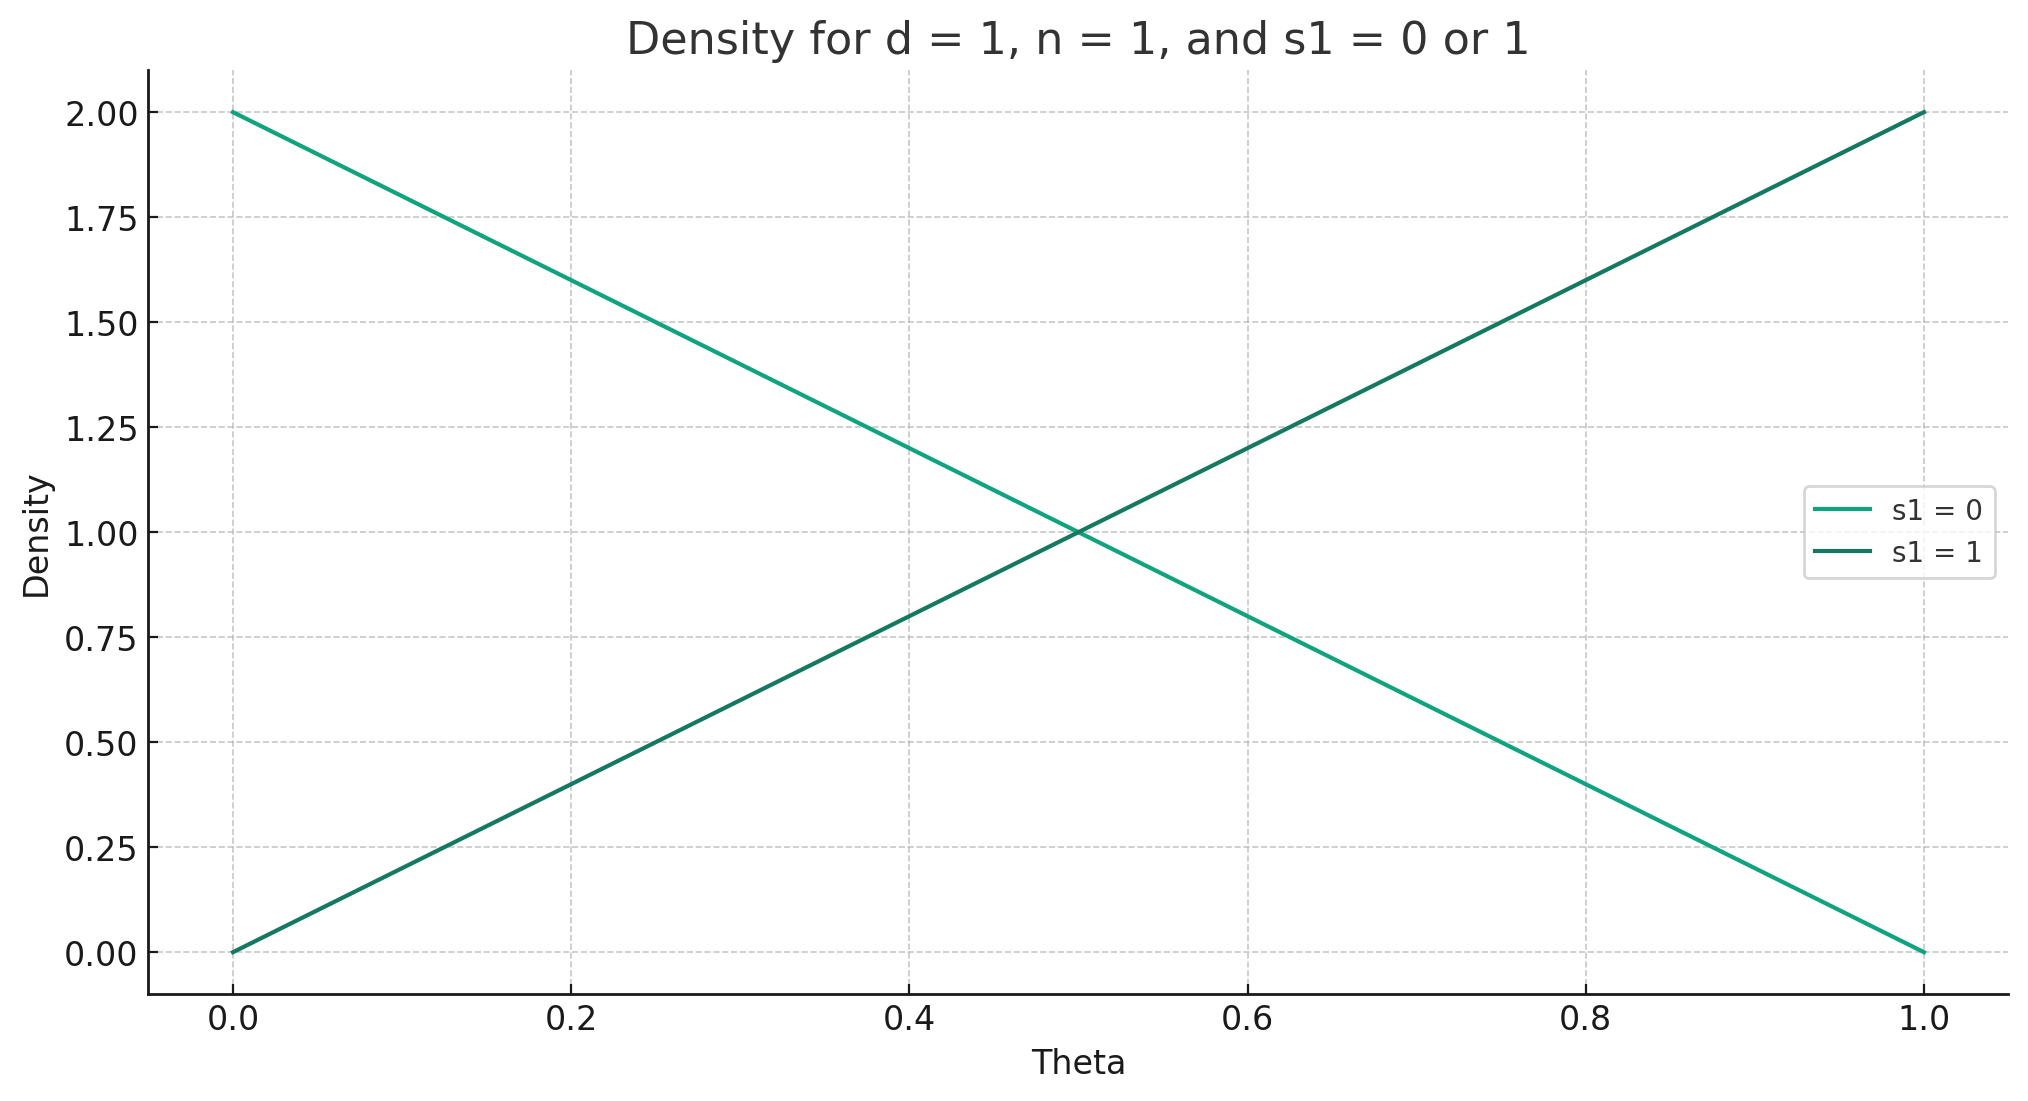
\includegraphics[width=\textwidth]{Q2c}
    \end{center}
    Note that an observation of $0$ turns the uniform distribution into a distribution that weighs a lot more on smaller $\theta$, and vice versa.

    \item
    Integrate the product $P_{X|\Theta}(x|\theta)P_{\Theta|T}(\theta|\D)$ over $\theta$ to obtain the desired conditional probability. \\

    \textbf{Solution}

    \begin{align*}
      P_{X|T}(\mathbf{x}|D)
      &= \int_0^1  P_{X|\Theta}(x|\theta)P_{\Theta|T}(\theta|\D) d \theta \\
      &= \int_0^1 \prod_{i = 1}^d \theta^{x_i}_i (1 - \theta_i)^{1 - x_i} \cdot \frac{(n + 1)!}{s_i!(n - s_i)!} \theta_i^{s_i}(1 - \theta_i)^{n - s_i} \\
      &= \prod_{i = 1}^d \frac{(n + 1)!}{s_i!(n - s_i)!} \int_0^1 \theta^{x_i + s_i}_i (1 - \theta_i)^{n - x_i - s_i + 1} \\
      &= \prod_{i = 1}^d \frac{(n + 1)!}{s_i!(n - s_i)!} \cdot \frac{(x_i + s_i)!(n - x_i - s_i + 1)!}{(n + 2)!} \\
      &= \prod_{i = 1}^d \frac{(s_i + 1)^{x_i}(n - s_i + 1)^{1 - x_i}}{n + 2} \\
      &= \prod_{i = 1}^d \left(\frac{s_i + 1}{n + 2}\right)^{x_i}\left(1 - \frac{s_i + 1}{n + 2}\right)^{1 - x_i}.
    \end{align*}

    \item
    If we think of obtaining $P_{X|T}(\mathbf{x}|\D)$ by substituting an estimate $\hat{\theta}$ for $\theta$ in $P_{X|\Theta}(x|\theta)$, what is the effective Bayesian estimate for $\theta$. \\

    \textbf{Solution} 

    The effective estimate for $\theta$ is
    \[
      \hat{\theta_i} = \frac{s_i + 1}{n + 2},
    \]
    for $i \in \{1, \dots, d\}$. \\
  \end{enumerate}

  \part{B}

  What is the ML estimate for $\theta$ in this problem? What is the MAP estimate for $\theta$ in this problem? Do you see any advantage in favoring one of the estimates in favor of the others? How does that relate to the uniform prior that was assumed for $\theta$? \\

  \textbf{Solution} 
  
  The ML estimate is
  \begin{align*}
    \theta_{ML}
    &= \underset{\theta}{\arg \max} \, P_{T|\Theta}(\D|\theta) \\
    &= \underset{\theta}{\arg \max} \, \prod_{i = 1}^d \theta^{s_i}_i(1 - \theta_i)^{n - s_i} \\
    &= \underset{\theta}{\arg \max} \, \sum_{i = 1}^d s_i \ln \theta_i + (n - s_i) \ln(1 - \theta_i).
  \end{align*}
  Let $g(\theta) = \sum_{i = 1}^d s_i \ln \theta_i + (n - s_i) \ln(1 - \theta_i)$. Since $\frac{\partial g}{\partial \theta_i} = \frac{s_i}{\theta_i} - \frac{n - s_i}{1 - \theta_i}$ and $\frac{\partial^2 g_i}{\partial \theta_i^2} = -\frac{s_i}{\theta_i^2} - \frac{n - s_i}{(1 - \theta_i)^2} < 0$, we get $\theta_{ML} = \frac{1}{n}\mathbf{s}$.
  
  The MAP estimate is
  \begin{align*}
    \theta_{MAP}
    &= \underset{\theta}{\arg \max} \, P_{T|\Theta}(\D|\theta)P_{\Theta}(\theta) && (P_{\Theta}(\theta) \text{ is uniform}) \\
    &= \underset{\theta}{\arg \max} \, P_{T|\Theta}(\D|\theta) \\
    &= \theta_{ML}.
  \end{align*}
  We can see that our assumption of the uniform prior made the two estimates identical, and thus there are no advantage favoring one over another in this case.
\end{homeworkProblem}

\pagebreak

\begin{homeworkProblem}
  Consider problem 3 of the previous assignment, i.e. a random variable $X$ such that $P_X(k) = \pi_k, k \in {1, \dots , N}$, $n$ independent observations from $X$, a random vector $C = (C_1,\dots , C_N)^T$ where $C_k$ is the number of times that the observed value is $k$ (i.e. $C$ is the histogram of the sample of observations). We have seen that, $C$ has multinomial distribution
  \[
    P_{C_1,\dots,C_N}(c_1,\dots,c_N) = \frac{n!}{\prod_{k = 1}^N c_k!}\prod^N_{j = 1}\pi^{c_j}_j.
  \]
  In this problem we are going to compute MAP estimates for this model. Notice that the parameters are probabilities and, therefore, not every prior will be acceptable here (since $\pi_j > 0$ and $\sum_j \pi_j = 1$ for the prior to be valid). One distribution over vectors $\pi = (\pi_1, \dots , \pi_N)^T$ that satisfies this constraint is the Dirichlet distribution
  \[
    P_{\Pi_1,\dots,\Pi_N}(\pi_1,\dots,\pi_N) = \frac{\Gamma \left(\sum^N_{j = 1} u_j\right)}{\prod_{k = 1}^N \Gamma(u_j)}\prod^N_{j = 1}\pi^{u_j - 1}_j,
  \]
  where the $u_j$ are the set of $hyperparameters$ (parameters of the prior) and
  \[
    \Gamma(x) = \int^{\infty}_0 e^{-t}t^{x - 1} dt
  \]
  the Gamma function. \\

  \part{A}

  Derive the MAP estimator for the parameters $\pi_i, i = 1,\dots , N$ using the Dirichlet prior. \\

  \textbf{Solution}

  Let $\mathbf{\pi} = (\pi_1, \dots, \pi_N)$.
  \begin{align*}
    \mathbf{\pi}^*
    &= \underset{\mathbf{\pi}}{\arg \max} \, P_{C_1,\dots,C_N | \Pi}(c_1,\dots,c_N | \pi)P_{\Pi_1,\dots,\Pi_N}(\pi_1,\dots,\pi_N) \\
    &= \underset{\mathbf{\pi}}{\arg \max} \, \frac{n!\Gamma \left(\sum^N_{j = 1} u_j\right)}{\prod_{k = 1}^N c_k!\Gamma(u_j)} \prod^N_{j = 1}\pi^{c_j + u_j - 1}_j \\
    &= \underset{\mathbf{\pi}}{\arg \max} \, -\sum_{j = 1}^N (c_j + u_j - 1) \ln \pi_j.
  \end{align*}
  Let $g(\pi) = -\sum_{j = 1}^N (c_j + u_j - 1) \ln \pi_j - \lambda\left(\sum_{j = 1}^N \pi_j - 1\right)$. Since $\frac{\partial g}{\partial \pi_j} = \frac{c_j + u_j - 1}{\pi_j} - \lambda$ and $\frac{\partial^2 g}{\partial \pi_j^2} = -\frac{c_j + u_j - 1}{\pi_j^2} < 0$, we know $c_j + u_j - 1 = \lambda\pi_j$. Summing over $j$, we get $\lambda = n - N + \sum_j u_j$, and so $\pi_j^* = \frac{c_j + u_j - 1}{\lambda} = \frac{c_j + u_j - 1}{n + \sum_j u_j - N}$.
  
  \pagebreak

  \part{B}

  Compare this estimator with the ML estimator derived in the previous assignment. What is the use of this prior equivalent to, in terms of the ML solution? \\

  \textbf{Solution}

  Since $\lim\limits_{n \to \infty} \pi^*_j = \frac{c_j}{n + \sum_j u_j - N}$, we know $\lim\limits_{n \to \infty} \frac{\pi^*_j}{{\pi_{MAP}}_j} = \frac{n + \sum_j u_j - N}{n} = 1$, and thus $\pi^*$ approaches the ML estimate when $n$ grows large. Conversely, when $n = 0$, $\pi^*_j = \frac{u_j - 1}{\sum_j u_j - N}$. Thus, we can interpret $c_j$ and $n$ as the observed counts and trails, and view $u_j - 1$ and $\sum_j u_j - N$ as the supposed counts and trails from our knowledge. \\

  \part{C}

  What is the effect of the prior as the number of samples $n$ increases? Does this make intuitive sense? \\

  \textbf{Solution}

  From part B, we see that the MAP estimate appraoches the ML estimate when $n$ grows large. This means that the prior becomes a lot less influencial compared to our estimation when the sample size is large, which aligns with the idea of Bayesian estimation. \\

  \part{D}

  In this problem and problem 2 we have seen two ways of avoiding the computational complexity of computing a fully Bayesian solution: i) to rely on a non-informative prior, and ii) to rely on an informative prior and compute the MAP solution. Qualitatively, what do you have to say about the results obtained with the two solutions? What does this tell you about the robustness of the Bayesian framework? \\

  \textbf{Solution}

  Regardless of the prior, the Bayesian framework is qualitatively equivalent to the ML estimate when $n$ is large, which implies that the Bayesian framework is really robust.

\end{homeworkProblem}

\end{document}